% !LW recipe = latexmk (latexmkrc)
% Writing sample ported from write-up/Thesis Abridged.docx.
% Build: latexmk (see latexmkrc), or xelatex -> biber -> xelatex x2.
% (The line above makes VS Code's LaTeX Workshop build with latexmk + latexmkrc, so
% biber runs and aux files go to build/. Do not use "% !TEX program = xelatex": it
% makes LaTeX Workshop run a single xelatex pass, which leaves citations and new
% cross-references undefined.)
%
% Conventions used in this file:
%   \todo{...}      visible red note for something to fix before submission;
%                   set \showtodosfalse below to hide all of them.
%   % COMMENT (...) advisor comments carried over from the .docx, at their anchor point.
%   % PORT: ...     note on a change made during the port.

\documentclass[12pt,letterpaper]{article}

% ---------- Page layout ----------
\usepackage[margin=1in]{geometry}
\usepackage{setspace}
\doublespacing

% ---------- Fonts (XeLaTeX) ----------
\usepackage{amsmath}
\usepackage{newtxmath}
\usepackage{fontspec}
\setmainfont{texgyretermes}[
  Extension      = .otf,
  UprightFont    = *-regular,
  BoldFont       = *-bold,
  ItalicFont     = *-italic,
  BoldItalicFont = *-bolditalic]
\usepackage{xeCJK}
\setCJKmainfont{Songti SC}

% ---------- Figures and tables ----------
\usepackage{graphicx}
\graphicspath{{../../figures/output/}}
\usepackage{booktabs}
\usepackage{threeparttable}
\usepackage[font=small,labelfont=bf,skip=6pt]{caption}
\usepackage{float}
\usepackage[section]{placeins}  % floats never drift past the end of their section
% Float placement: LaTeX's defaults (a float may fill at most 70% of a text page, at
% least 20% of a page must be text, a float-only page must be 50% full) push mid-sized
% figures off the page that cites them. Relax them so a figure lands where it is cited
% when it fits, and otherwise at the top of the next page.
\renewcommand{\topfraction}{0.9}
\renewcommand{\bottomfraction}{0.8}
\renewcommand{\textfraction}{0.07}
\renewcommand{\floatpagefraction}{0.8}
\setcounter{topnumber}{3}
\setcounter{bottomnumber}{2}
\setcounter{totalnumber}{4}

% ---------- Headings ----------
\usepackage{titlesec}
\titleformat{\section}{\normalfont\large\bfseries}{\thesection.}{0.6em}{}
\titleformat{\subsection}{\normalfont\normalsize\bfseries}{\thesubsection}{0.6em}{}
\titleformat{\subsubsection}{\normalfont\normalsize\itshape}{\thesubsubsection}{0.6em}{}
\titlespacing*{\section}{0pt}{1.2\baselineskip}{0.4\baselineskip}
\titlespacing*{\subsection}{0pt}{0.8\baselineskip}{0.2\baselineskip}
\titlespacing*{\subsubsection}{0pt}{0.6\baselineskip}{0.1\baselineskip}
\setcounter{secnumdepth}{2}

% ---------- Quotes and citations ----------
\usepackage[english]{babel}
\usepackage{csquotes}
\AtBeginEnvironment{displayquote}{\singlespacing}
\usepackage[authordate,backend=biber,noibid,natbib=false]{biblatex-chicago}
\addbibresource{references.bib}
% Let long URLs break anywhere instead of stretching inter-word spacing.
\setcounter{biburlnumpenalty}{100}
\setcounter{biburlucpenalty}{100}
\setcounter{biburllcpenalty}{100}

% ---------- Misc ----------
\usepackage{microtype}
\usepackage{xcolor}
\usepackage[hidelinks]{hyperref}
\usepackage[capitalise,noabbrev]{cleveref}

\newif\ifshowtodos
\showtodostrue
\newcommand{\todo}[1]{\ifshowtodos{\color{red}\footnotesize[\textsc{todo}: #1]}\fi}

\title{\textbf{Words That Will Shake the World:}\\[0.3em]
  \large Investigating the Interaction between US and Chinese Foreign Policy Discourse with Sentiment Analysis and Granger Causality Tests}
\author{Alexander Lin\thanks{Adapted from an honors thesis in International Politics, Edmund A. Walsh School of Foreign Service, Georgetown University (2023), advised by Professor Lisa Singh. An interactive visualization of Chinese and US rhetorical sentiments over time is available at \url{https://alexlin.shinyapps.io/Thesis_Visualization/}.}}
\date{}

\begin{document}

\begin{singlespace}
\maketitle
\end{singlespace}

\begin{abstract}
\noindent
As tensions continue to rise between China and the US, constructive dialogue has been crowded out by tit-for-tat recriminations. This paper seeks to explore the patterns of interaction between US and Chinese foreign policy discourse in the context of this trend. Specifically, it applies data-driven methods to investigate whether Chinese political discourse vis-à-vis the US is reactive to US rhetoric about China---and vice versa---between 2002 and 2021.

I pair Chinese Ministry of Foreign Affairs press conference transcripts and \emph{People's Daily} publications with over 35,000 US documents mentioning China from the Presidential Library and Congressional databases. Lexicon-based and supervised machine learning models then classify the sentiments of these texts. Subsequently, I construct time series of locally averaged sentiments and apply Granger causality tests to determine whether one country's discursive patterns can predict those of its counterpart. 

This paper finds consistent evidence for unidirectional Granger causality with US data as a response, indicating that China seems to initiate rhetorical reconciliation and hostilities more often, while the US plays a more reactive role in bilateral discourse. 
\end{abstract}

% =====================================================================
\section{US-China Relations at a Crossroads}
\label{sec:intro}

As the geopolitical fault lines between the US and China harden, their bilateral relations have become increasingly defined by mutual accusations and vitriol. Whereas good-faith dialogue takes the edge off rising tensions and lays the groundwork for more constructive diplomatic engagement (as was the purpose of the Bush-era Strategic Economic Dialogue and its Obama-era successor, the Strategic and Economic Dialogue), tit-for-tat rhetorical jousting erodes trust and engenders a cycle of aggressive posturing. The hostile rhetoric that dominated the high-level Anchorage summit in 2021, as well as outbursts from ``Wolf Warrior'' diplomats, demonstrates the corrosive effects of virulent dialogue.

Given that words can make or break bilateral relations, being able to effectively parse, understand, and even forecast how Beijing speaks about the US is a central priority for scholars of US-China relations. A wide body of literature has explored various elements of China's foreign policy discourse, ranging from motifs like ``tianxia'' (天下), to how historical grievance animates language, to Hu Jintao's mantras ``harmonious society'' and ``harmonious world,'' to the ubiquitous Xi-era slogan ``community of common destiny,'' to the ``Wolf Warrior'' phenomenon \autocites{callahan2007}{zheng2007}{wang2014}{sullivan2023}.

However, existing research faces two important limitations. First, it rarely traces Chinese rhetoric as a product of interaction with---or a response to---American foreign policy discourse over an extended time frame.\footnote{Some studies do examine discursive interactions within particular time periods or issue areas; see, e.g., \textcite[295]{jaworsky2021}.} Indeed, discourse does not materialize in a vacuum, but is rather a series of stimuli and responses that are shaped and reshaped through an iterative, interactive process. What's more, researchers often have to concentrate their analysis on just a few texts, making it difficult to glean insights about more holistic trends within the US-China discursive landscape, which encompasses hundreds of thousands of texts churned out over multiple decades.\footnote{Nevertheless, some quantitative papers that look at larger pools of foreign policy discourse do exist and prove helpful. See \textcite{mokry2024}.}

My paper attempts to partially address these limitations by exploring how American foreign policy discourse vis-à-vis China interacts and correlates with Chinese discourse about the US. More specifically, I ask whether it is possible to pinpoint a ``trend-setter'' and a ``trend-reactor'' in the sentiments of US and Chinese government (and media) discourses vis-à-vis each other. If so, who more often plays the role of the sentiment ``trend-setter,'' and who plays the role of the ``trend-reactor''?

% PORT: Figure 1 (hypothesized interaction patterns) was cut; the closing
% parenthetical "(as illustrated in Figure 1)" was removed from this paragraph.
To situate this research query within a quantitative space, I aim to transform vast corpora of US and Chinese foreign policy discourse into sentiment ``scores'' over time. In other words, every relevant text is assigned a numerical score that places its sentiment (or tone) along a linear spectrum ranging from negative to positive. These numeric proxies for sentiment are then averaged to create time series. Subsequently, I examine whether there exists a ``lagged correlation'' between the sentiment time series corresponding to US and Chinese rhetoric.

% =====================================================================
\section{Data}
\label{sec:data}
% COMMENT (Berlinerblau): One observation. Right before 9/11 the US shot down a
% Chinese plane and the pilot died. This led to a lot of shittalking. Then 9/11
% happened and everyone forgot. Does this case interest you?

\subsection{Data Collection}

\subsubsection*{Chinese Data}

Data on Chinese foreign policy discourse came ready-made. Mochtak and Turcsanyi curated the Chinese Ministry of Foreign Affairs Press Conferences Corpus. This dataset contains roughly 23,000 question-answer dyads, ranging from October 2002 to December 2021, that were extracted from press conference transcripts published on the MFA's English website \autocite{mochtak2022data}.

A vast collection of English \emph{People's Daily} publications, provided by Fisher and Klein through the FOCUSdata project, supplemented the MFA corpus to round out my Chinese foreign policy dataset. The \emph{People's Daily} corpus captures 190,000 articles ranging from May 2007 to December 2020 \autocite{fisher2022data}.\footnote{For more details on how the FOCUSdata project collected its vast datasets, and how it conducted preliminary sentiment analysis, see \textcite{fisher2022focus}.}

\subsubsection*{US Data}

Pre-existing datasets that trace US foreign policy rhetoric are scant, if they exist at all. This means that an original data collection endeavor is warranted. In order to maximize congruence between the China and US data, the intuitive source of documents here would have been State Department press releases. However, these transcripts are scattered across multiple archived websites with non-uniform interfaces corresponding to the Clinton, Bush, Obama, and Trump presidencies. I therefore drew instead on HeinOnline's federal government databases.

% PORT: "HeinOnline's Congressional compiled another dataset" -> added the missing
% "Documents database and".
Using a custom scraper built on Selenium ChromeDriver, I compiled all documents that included the named entities ``China,'' ``Chinese,'' ``CCP,'' and ``PRC'' within HeinOnline's Presidential Libraries since 2000 \autocite{heinPresidential}. The custom dataset pooled together roughly 4,800 entries sourced from the Daily Compilation of Presidential Documents and the Public Papers of five administrations, almost all of which are transcripts of the President's public statements. A similar scraper searched HeinOnline's Congressional Documents database and compiled another dataset totaling nearly 30,300 documents, drawn primarily from Congressional Research Service (CRS) reports and roughly fourteen volumes of the \emph{Congressional Record}, which documents daily proceedings on the Senate and House floors \autocite{heinCongress}.

% PORT: this heading read "Data Collection" (a duplicate) in the .docx; the full
% thesis calls this subsection "Data Cleaning".
\subsection{Data Cleaning}

\subsubsection*{Chinese Data}

The first step in the Chinese data cleaning pipeline was to extract each entry within the MFA and \emph{People's Daily} datasets that directly mentioned the United States (or its acronyms, ``US,'' or ``U.S.'').

Moreover, the MFA is much closer to China's foreign policy-making process than \emph{People's Daily} and is thus a more authoritative representation of Beijing's true posture towards the US. I therefore keep every relevant MFA document and supplement them with a random sample of approximately 2,500 \emph{People's Daily} articles.

\Cref{fig:china-doc-freq} shows the number of documents mentioning the US in the MFA and \emph{People's Daily} corpora over time, after both corpora have been cleaned and trimmed by this pipeline.

\begin{figure}[!htbp]
  \centering
  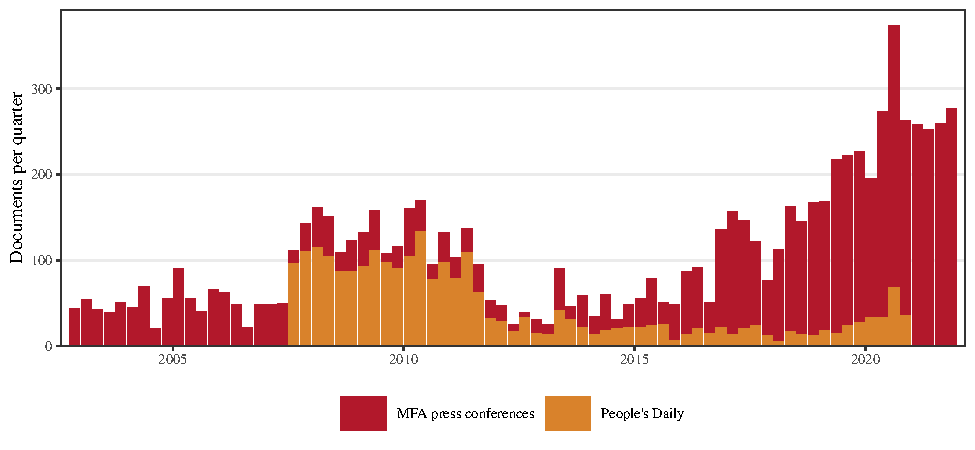
\includegraphics[width=\textwidth]{03_china_doc_frequency.pdf}
  \caption{Relevant document frequency, China data}
  \label{fig:china-doc-freq}
\end{figure}

\subsubsection*{US Data}

Because the White House holds the reins of foreign policy, whereas Congress often takes on the role of a rowdy passenger, the US sample is weighted in the same way: the combined US dataset privileges Presidential data and incorporates all of its dated entries. It then supplements documents from the Presidential Library with a random sample of 2,000 Congressional data points. \Cref{fig:us-doc-freq} traces the frequency of US documents over time, disaggregated by the compilation or archive from which they originated.

\begin{figure}[!htbp]
  \centering
  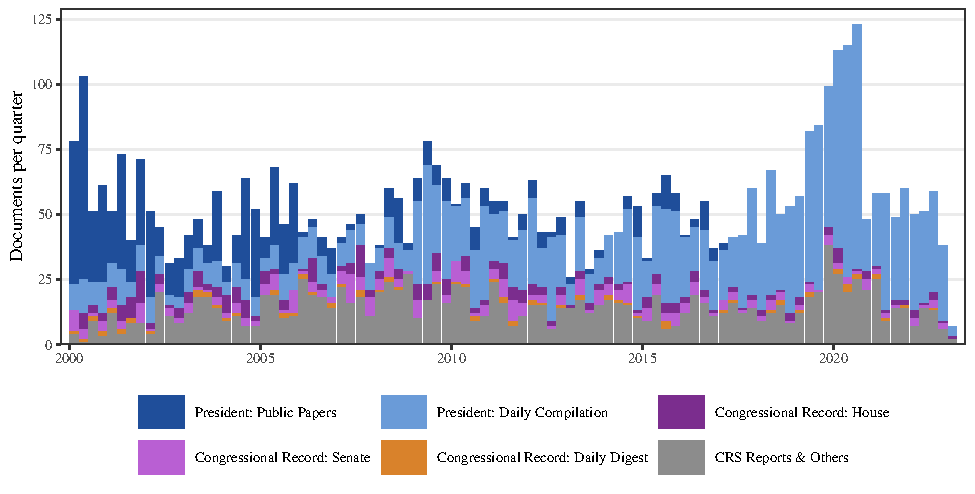
\includegraphics[width=\textwidth]{02_us_doc_frequency.pdf}
  \caption{Relevant document frequency, US data}
  \label{fig:us-doc-freq}
\end{figure}

\Cref{fig:composition} illustrates the composition of the fully-processed US and China datasets. Overall, around 15,200 texts are used in subsequent analyses, of which 6,000 are sourced from the MFA, 2,480 are sampled from \emph{People's Daily}, 4,760 are derived from the Presidential Library, and 2,000 are sampled from Congress. The next section describes how these documents are scored for sentiment and aggregated into time series.

\begin{figure}[!htbp]
  \centering
  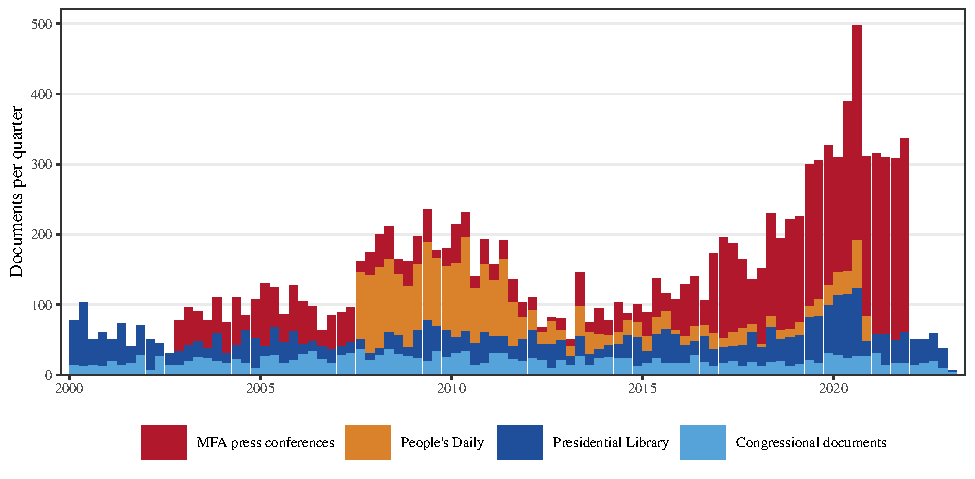
\includegraphics[width=\textwidth]{04_data_composition.pdf}
  \caption{Composition of relevant data}
  \label{fig:composition}
\end{figure}

% =====================================================================
\section{Methodology}
\label{sec:methods}

\subsection{Extracting a Country's Latent Posture from Rhetoric}

For each document $d$ produced in country $c$ that mentions its counterpart $c'$, issued by speaker or data source $k(d)$ in period $t(d)$, it is possible to represent the sentiment $y_d$ of $d$ as the sum of three terms: (1) $c$'s latent posture towards $c'$ in period $t(d)$, denoted by $\theta_{c,t(d)}$, (2) a time-invariant speaker or source effect $\alpha_{k(d)}$, and (3) a random error term, $\varepsilon_{d}$:
\begin{align}
  y_d = \theta_{c,t(d)} + \alpha_{k(d)} + \varepsilon_d .
  \label{eq:doc}
\end{align}
Here, $\alpha_{k(d)}$ captures the idiosyncratic posture of the speaker, the style of the data source, or any systematic bias a sentiment classifier has towards a particular text genre.

Averaging sentiment across all $n_{c,t}$ documents that country $c$ produces in period $t$ yields the following expression:
\begin{align}
  \bar y_{c,t} = \theta_{c,t} + \underbrace{\sum_k w_{k,t}\,\alpha_k}_{\text{doc composition}} + \bar\varepsilon_{c,t},
\qquad w_{k,t} = n_{k,t}/n_{c,t}.
  \label{eq:avg}
\end{align}
This paper estimates $\theta_{c,t}$ for successive weeks or months by averaging the sentiment scores of all relevant documents within each period. It then constructs a time series of these estimates, $\{\bar y_{c,t}\}_{t=1}^T$, for each country $c$ and examines whether the Chinese time series reacts to the US time series, or vice versa.

Because $\bar y_{c,t}$ also moves with the document composition term in \cref{eq:avg}, it may be advisable to subtract that term out of the average sentiment. This ensures that the estimates of $\theta_{c,t}$ are not confounded by a change in document genre or speaker composition. For example, a sudden influx of documents from \emph{People's Daily} around 2007, as observed in \Cref{fig:china-doc-freq}, might skew the average sentiment even when China's latent posture remains unchanged. An adjusted average sentiment $\tilde y_{c,t}$ can be represented as follows:
\begin{align}
  \tilde y_{c,t} = \bar y_{c,t} - \sum_k w_{k,t}\hat\alpha_k
\end{align}
However, two considerations moderate the usefulness of $\tilde y_{c,t}$. First, speaker or source effects are poorly identified when most or all documents in $t$ are issued by the same speaker or source. Second, these effects may be endogenous to posture. A more hawkish Chinese posture towards the US, for instance, can manifest as more frequent podium appearances of ``Wolf Warrior'' spokespeople like Zhao Lijian. 

My analysis finds that subtracting out the document composition term does not substantially move average sentiments over time, except in the Chinese series before \emph{People's Daily} documents enter the sample in mid-2007, as illustrated in \cref{fig:speaker-fe}. The Granger causality test results are robust to either time series construction. For the sake of simplicity, this paper will present results using $\bar y_{c,t}$.

\begin{figure}[!htbp]
  \centering
  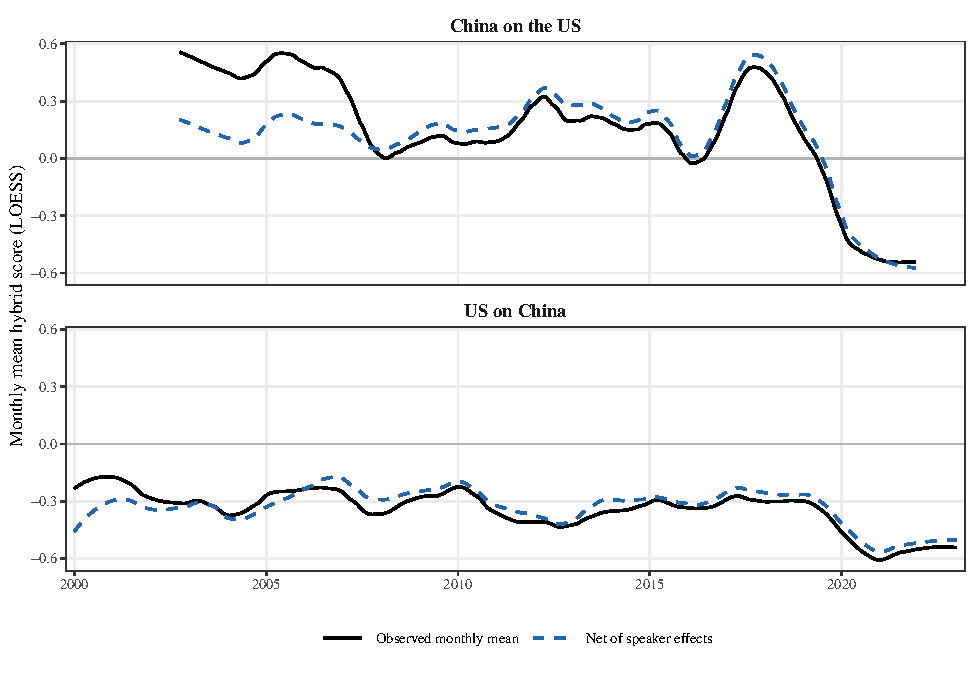
\includegraphics[width=\textwidth]{../../robustness/output/speaker_fe_series.pdf}
  \caption[Chinese and US sentiments net of speaker effects]{Chinese and US sentiments net of speaker effects. Solid: observed monthly mean sentiment $\bar y_{c,t}$; dashed: adjusted series $\tilde y_{c,t}$, with speaker effects $\hat\alpha_k$ (MFA spokesperson, \emph{People's Daily}, Presidential Library archive, Congressional Record section or CRS) estimated jointly with month fixed effects, so that each $\hat\alpha_k$ is identified only from speakers active in the same month. Full country series, approach 2 scores; curves are LOESS fits (span 0.15).}
  \label{fig:speaker-fe}
\end{figure}

\subsection{Refining the Research Question}
\label{sec:refine}

Given the thematic diversity and volatility of the US and Chinese foreign policy discursive landscape, it would be overly reductive to crowd all textual data from the US and China into just two time series. As such, the central research question must be broken down into two more manageable components.

First, we want to zero in on narrower time frames within broader sentiment trends. This means making longitudinal (i.e.\ temporal) cuts to the textual data and scanning for more local---rather than global---lagged correlations.

Second, it is advisable to examine how the patterns of interaction between US and Chinese discourse vary by foreign policy issue areas. Are there particular topics that prompt the US or China to take the rhetorical reins and set sentiment trends, whereas in other topics, the former trend-setter slips into a more reactive role? This entails partitioning the textual datasets by topic.

\subsection{Sentiment Analysis}

A growing number of studies apply sentiment analysis to US-China relations. \Textcite{mochtak2021}, who created the MFA press corpus, leveraged the Bing Liu lexicon to conduct some exploratory analysis of sentiment polarity on the MFA dataset. \Textcite[403--406]{zeng2022} started from a premise related to my own research question, whereby the authors sought to regress sentiment scores of US news media based on the Bing Liu lexicon (which acts as a proxy for US-China tensions) against US imports and disruptions to the global value chain during the trade war. Research by \textcite{choi2023}, moreover, uses the AFINN lexicon to compare the sentiments of speeches from members of Congress regarding the US's ratification of two free trade agreements. Although only tangentially related to the study of US-China relations, it nevertheless shows that sentiment analysis can be applied to official government discourse.

These studies, however, overwhelmingly rely on a lexicon-based approach, which assigns texts sentiment polarities by comparing their features to a pre-existing valence dictionary. This family of sentiment analysis methods is very ``economical,'' in that it derives satisfactory results with a minimal computational load. The disadvantage here, however, is that the dictionaries we use might not be well-adapted to specialized vocabulary, such as diplomatic talking points and domain-specific jargon.

As such, my research opts for a ``hybrid'' approach, whereby I pair the Bing Liu lexicon method with supervised machine learning approaches. This entails manually coding a random sample of 1,200 texts (600 from each country) into three classes (``positive,'' ``negative,'' or ``ambiguous''), transforming the documents into term-document matrices (TDMs) weighted by TF-IDF, and then allowing my algorithm to ``infer'' the functions that best classify sentiments on the TDMs under a stratified train-test split. These trained classifiers could then assign sentiment scores to the entire textual corpora. Supervised learning here is advisable because it tailors my sentiment analysis algorithm to consider specialized, foreign policy-oriented vocabulary that might be less compatible with traditional valence lexicons.\footnote{For a comparison of the pros and cons of lexicon-based and learning methods, see \textcite{kolchyna2015} and \textcite[444--45]{verma2018}.} Specifically, I implemented four supervised learning models: random forest, decision trees, Naive Bayes, and support vector machines (SVMs). The SVM and random forest models performed the best. The final hybrid score is an ensemble average of the SVM label, the random forest label, and the standardized Bing Liu lexicon score.\footnote{For the viability of hybrid models, see \textcite{dandrea2015}.}

The hardest class of documents to classify is the one with ambiguous sentiments. I apply three different training approaches to see which addresses this challenge most effectively. The first approach performed an 80-20 train-test split on only the positive and negative documents in the manually coded sample. The second approach included all three sentiment categories (adding a random sample of 75 ambiguous documents). The third approach recoded the three-category sentiment label as two binary indicators, $\mathbf{1}\{d \text{ is positive}\}$ and $\mathbf{1}\{d \text{ is negative}\}$, and trained a separate model on each.

\subsection{Granger Causality}

\subsubsection*{The Mechanics of a Granger Test}

Since this paper revolves around the central research question of whether one country's discourse takes the role of a sentiment ``trend-setter,'' while its counterpart acts as a ``trend-reactor,'' it may be particularly fruitful to borrow a tool that is ubiquitous---if often over-interpreted---in time series econometrics. Specifically, this paper will apply Granger causality to assess whether the patterns of interaction between the US and Chinese sentiments are statistically significant.

The test essentially looks at whether the predictive power of a time series (such as US sentiment trends) can be significantly improved by expanding a restricted, strictly autoregressive model to include lagged values of another time series (for example, Chinese sentiment) as regressors. The univariate (restricted) and bivariate (full) models are:
\begin{align}
  \text{Restricted:}\quad \bar{y}_{\mathrm{US},t} &= \mu + \sum_{n=1}^{p} \gamma_n \bar{y}_{\mathrm{US},t-n} + u_t \\
  \text{Full:}\quad \bar{y}_{\mathrm{US},t} &= \mu + \sum_{n=1}^{p} \gamma_n \bar{y}_{\mathrm{US},t-n} + \sum_{n=1}^{p} \beta_n \bar{y}_{\mathrm{CN},t-n} + v_t
\end{align}
Here, $\bar{y}_{\mathrm{US},t}$ denotes US sentiment towards China in period $t$, while $\bar{y}_{\mathrm{US},t-n}$ (or $\bar{y}_{\mathrm{CN},t-n}$) denotes US (or Chinese) sentiment in period $t-n$. In this sense, $p$ is the ``lag order'' of the Granger test, or the number of past periods we consider to model the sentiment in period $t$. $u_t$ and $v_t$ are the error terms of the restricted and full models, respectively. The null hypothesis that Chinese sentiment does not Granger-cause US sentiment is $\beta_1 = \dots = \beta_p = 0$.

To test this null, I use an F-test of whether the residual sum of squares (RSS) of the full model is significantly smaller than that of the restricted model. With $T$ observations used in the regressions, the F-statistic is
\begin{align}
  F = \frac{(\mathrm{RSS}_{\text{restricted}} - \mathrm{RSS}_{\text{full}}) / p}{\mathrm{RSS}_{\text{full}} / (T - 2p - 1)}.
\end{align}
Because we want to understand the lagged correlation between US and Chinese sentiments in both directions, I also flip the variables in the models above and run the test with the Chinese time series as the response.

\subsubsection*{Applying the Test to Different Cuts of Data}

Given the potentially reductive nature of analyzing global time series, this paper also applies time and topic filters to the textual datasets before implementing Granger tests (as motivated in \cref{sec:refine}).

Specifically, in order to narrow down the time frame of my analysis, I performed two types of ``cut'' on the data prior to inference testing: a ``backward-dating'' cut, which selects windows of monthly or weekly data before a certain date $D$, or a ``forward-dating'' cut, which extracts the portion of the original time series after $D$. The set of $D$ encompasses the start of every year from 2002 (the start of the Chinese time series) to 2020.

Alternatively, to achieve thematic---rather than temporal---granularity, this paper also looks at Granger causality for major topics (or themes) that dominate US-China foreign policy discourse. \Cref{tab:topic-keywords} lists each topic and the hand-picked keywords used to identify it.

% Topic-keyword dyads used to filter documents by issue area.
% Rebuilt from the table in "Thesis Abridged.docx" (Figure 6 there; Figure 11 in the full thesis).
\begin{table}[htbp]
\centering
\begin{threeparttable}
\caption{Topic--keyword dyads in US--China discourse}
\label{tab:topic-keywords}
\small
\begin{tabular}{@{}l l p{3.4in}@{}}
\toprule
 & Issue area & Keywords \\
\midrule
1 & Trade and finance & trade, tariff, protectionist, WTO, import, export, countervailing duty, intellectual property, manufactur(e/er/ing), jobs, exchange rate, currency (manipulation) \\
2 & Chinese domestic periphery & human rights, Xinjiang, Uyghur, Tibet, Hong Kong \\
3 & Taiwan & Taiwan \\
4 & Multilateral negotiations & denuclearize(ation), DPRK, North Korea, Iran, JCPOA, IAEA, Paris, climate, COP, ASEAN, APEC, EAS, G20, summit, multilateral \\
5 & South China Sea & South China Sea \\
6 & Global health and epidemics & COVID, coronavirus, pandemic, epidemic, outbreak, Ebola, SARS \\
7 & Russia & Russia \\
\bottomrule
\end{tabular}
\begin{tablenotes}[flushleft]
\footnotesize
\item \textit{Notes:} A document is assigned to every topic whose keywords it contains, so a document can belong to more than one topic.
\end{tablenotes}
\end{threeparttable}
\end{table}


\subsubsection*{Granger Causality Test Implementation}

To construct time series with a temporal cut, sentiment scores from both datasets are averaged by week or by month. On the other hand, sentiment scores for the time series with a thematic cut are grouped by month only. The reasoning here is that a topic filter makes the datasets much more ``shallow.'' In other words, grouping the data by weeks---as opposed to months---would create some time windows that are too sparsely populated by texts, or missing data entirely, to accurately reflect overarching rhetorical sentiments.

After constructing the weekly and monthly time series, I apply an Augmented Dickey-Fuller (ADF) test to every time series of interest in order to ensure compliance with the stationarity assumption of the Granger test. For pairs in which both series reject a unit root at the 5\% level, the Granger test is run on the series in levels. If neither series is stationary, I take first differences of both series before implementing further analyses. If only one series in the pair is stationary, however, first differencing both series over-differences the stationary one and costs statistical power. This motivates the modification proposed by \textcite{toda1995}, in which both series enter in levels with one additional lag included in the regression but excluded from the Wald test (computed in its F form).

To choose the lag order $p$, I examine how information criteria---such as the AIC (Akaike Information Criterion) and HQ (Hannan--Quinn) values---shift as this parameter is adjusted. Lag orders of 2 or 3 (in weeks or months, depending on the interval used to group the sentiment data) performed best. The main findings are robust to all lag orders $p \in \{1,\dots,5\}$.

% =====================================================================
\section{Results}
\label{sec:results}

\subsection{Sentiment Analysis}

The hybrid model generally classifies texts with positive or negative emotional valence well. Ambiguous sentiments, unsurprisingly, were more difficult to classify.

\Cref{fig:china-roc,fig:us-roc} report the performances of all three sentiment classification approaches on the Chinese and US datasets. Approach 2 (training the models once on all three sentiment classes) performed best on the US data, while approaches 1 and 3 did somewhat better on the Chinese data; approach 2 is the only one that performs well on both. A detailed report of sentiment classification results is provided in \cref{tab:sentiment-stats}. Subsequent time series analyses will use sentiment scores from this approach, although I also verified that the Granger causality test results are robust to the other two approaches.

% Generated by figures/06_sentiment_stats.R -- do not edit by hand.
% Requires \usepackage{booktabs} and \usepackage{threeparttable}.
\begin{table}[htbp]
\centering
\begin{threeparttable}
\caption{Performance of the hybrid sentiment classifier under three train-test approaches}
\label{tab:sentiment-stats}
\small
\begin{tabular}{l rrrrr @{\hspace{1.5em}} rrrrr}
\toprule
 & \multicolumn{5}{c}{China test data} & \multicolumn{5}{c}{US test data} \\
\cmidrule(lr){2-6} \cmidrule(lr){7-11}
\multicolumn{11}{l}{\textit{A. Three classes}} \\[2pt]
 & \multicolumn{3}{c}{F1} & Acc. & & \multicolumn{3}{c}{F1} & Acc. & \\
\cmidrule(lr){2-4} \cmidrule(lr){7-9}
 & Neg. & Amb. & Pos. & (\%) & $n$ & Neg. & Amb. & Pos. & (\%) & $n$ \\
\midrule
Approach 1 & 0.90 & 0.62 & 0.75 & 75.9 & 83 & 0.44 & 0.46 & 0.41 & 44.6 & 130 \\
Approach 2 & 0.79 & 0.40 & 0.76 & 69.9 & 73 & 0.84 & 0.39 & 0.63 & 68.6 & 70 \\
Approach 3 & 0.76 & 0.63 & 0.68 & 68.4 & 95 & 0.58 & 0.62 & 0.47 & 57.9 & 107 \\
\midrule
\multicolumn{11}{l}{\textit{B. One-vs-rest AUC and positive/negative accuracy}} \\[2pt]
 & \multicolumn{3}{c}{AUC} & Acc. & & \multicolumn{3}{c}{AUC} & Acc. & \\
\cmidrule(lr){2-4} \cmidrule(lr){7-9}
 & Neg. & Amb. & Pos. & (\%) & $n$ & Neg. & Amb. & Pos. & (\%) & $n$ \\
\midrule
Approach 1 & 0.96 & 0.56 & 0.91 & 91.4 & 58 & 0.64 & 0.50 & 0.75 & 80.0 & 55 \\
Approach 2 & 0.88 & 0.49 & 0.89 & 87.9 & 58 & 0.88 & 0.62 & 0.89 & 85.5 & 55 \\
Approach 3 & 0.96 & 0.56 & 0.87 & 92.9 & 56 & 0.74 & 0.54 & 0.80 & 78.0 & 50 \\
\bottomrule
\end{tabular}
\begin{tablenotes}[flushleft]
\footnotesize
\item \textit{Notes:} The hybrid score averages the SVM label, the random forest label and the standardized Bing Liu lexicon score.
Approach 1 trains on positive and negative documents only; approach 2 adds a sample of 75 ambiguous documents;
approach 3 trains separate positive-vs-not and negative-vs-not models and combines them.
Panel A: the continuous hybrid score is cut into three classes at quantiles matching the share of each hand-coded class in the evaluation set;
for approach 1, which has no ambiguous documents in its test split, held-out ambiguous documents are added to the evaluation set.
Panel B: AUC treats each class in turn as the outcome and the hybrid score as the predictor, with the direction of the score chosen for each class (the pROC default);
accuracy classifies hand-coded positive and negative documents by the sign of the hybrid score.
$n$ is the number of evaluation documents.
\end{tablenotes}
\end{threeparttable}
\end{table}


Under approach 2, the classification of positive- and negative-sentiment Chinese texts mentioning the US yielded AUCs of at least 0.88, although for texts containing ambiguous sentiments the AUC drops to 0.49, no better than chance. The corresponding ROC curves are laid out in \cref{fig:china-roc}. 

\begin{figure}[!htbp]
  \centering
  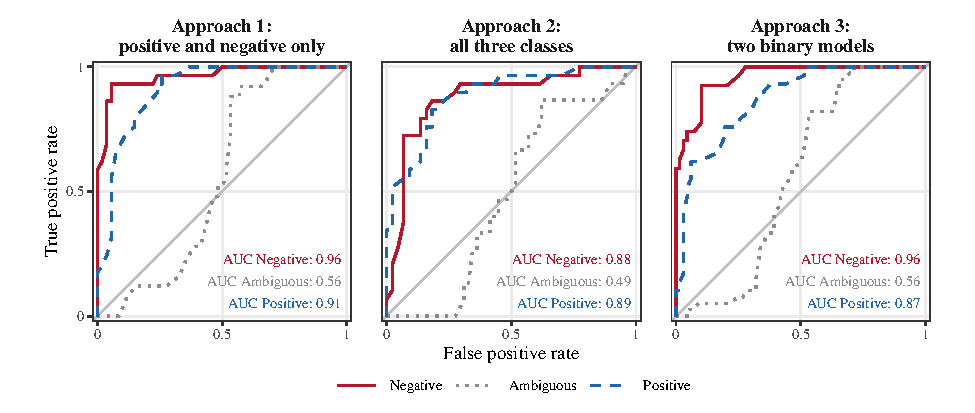
\includegraphics[width=\textwidth]{07_china_roc.pdf}
  \caption{ROC curves for sentiment classification of Chinese texts}
  \label{fig:china-roc}
\end{figure}

Meanwhile, for US texts mentioning China, the algorithm also achieved AUCs of at least 0.88 for positive and negative sentiments, compared to 0.62 for ambiguous sentiments (\cref{fig:us-roc}).

\begin{figure}[!htbp]
  \centering
  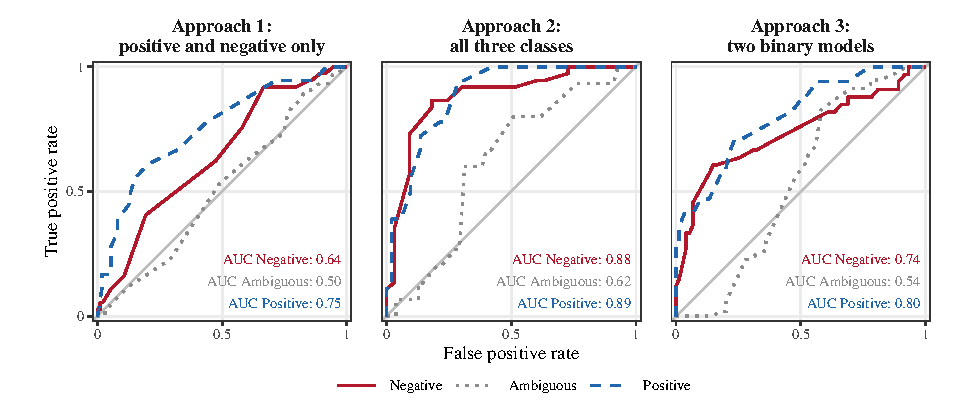
\includegraphics[width=\textwidth]{08_us_roc.pdf}
  \caption{ROC curves for sentiment classification of US texts}
  \label{fig:us-roc}
\end{figure}

Subsequently, by applying the sentiment classification algorithm to the entirety of the two textual datasets, and mapping the sentiment scores from each of the four datasets (i.e.\ MFA, \emph{People's Daily}, Presidential Library, and Congressional documents) onto distinct time series, we obtain \cref{fig:sent-source}. All four time series have been smoothed by LOESS.

\begin{figure}[!htbp]
  \centering
  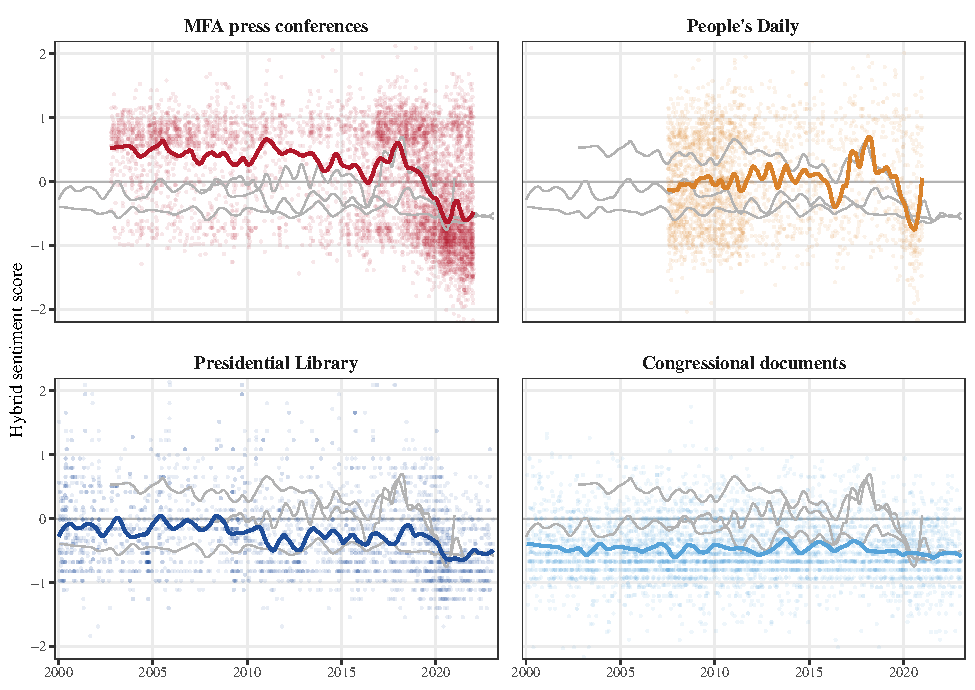
\includegraphics[width=\textwidth]{09_sentiment_by_source.pdf}
  \caption{Sentiments of each dataset over time}
  \label{fig:sent-source}
\end{figure}

We may also merge the datasets by country to create an aggregate Chinese time series and an aggregate US time series. To retain both local fluctuations and long-term trends, \cref{fig:sent-country} smooths each series with two different LOESS spans.

\begin{figure}[!htbp]
  \centering
  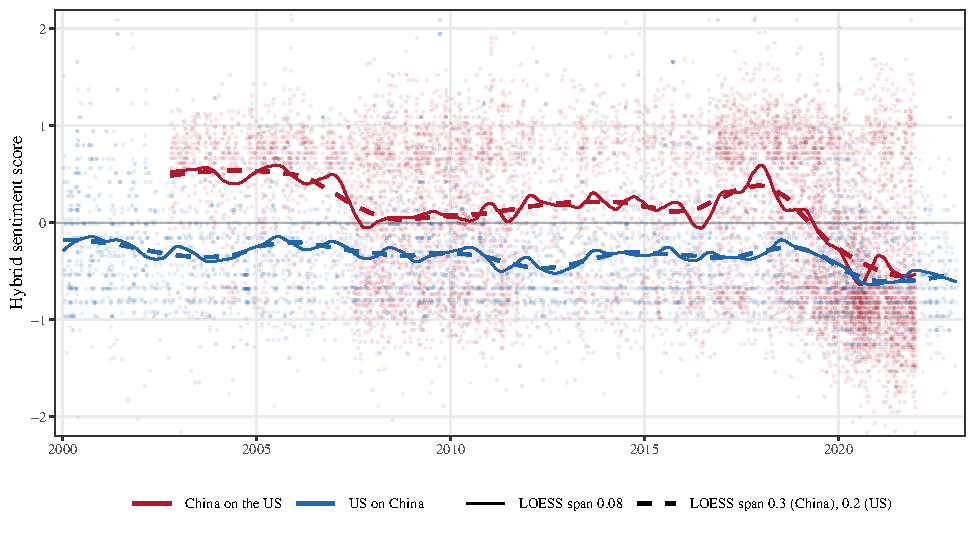
\includegraphics[width=\textwidth]{10_sentiment_by_country.pdf}
  \caption{Chinese and US sentiments over time}
  \label{fig:sent-country}
\end{figure}

Several insights can quickly be gleaned from \cref{fig:sent-source,fig:sent-country}. First, it is easy to pick up on the abnormally high degree of sentiment volatility roughly coinciding with the Trump presidency---particularly within the Chinese time series. Evan Medeiros terms this phenomenon the ``Trump bump.'' In the early days of the Trump presidency, Beijing softened its rhetoric in hopes of wooing the new administration that vowed to dismantle the Washington foreign policy establishment. This ostensible reconciliation culminated in Trump's state visit to Beijing in November 2017. Yet bilateral cordiality collapsed with the onset of a trade war. These events shaped the contours of the time series illustrated in \cref{fig:event-map}.

\begin{figure}[!htbp]
  \centering
  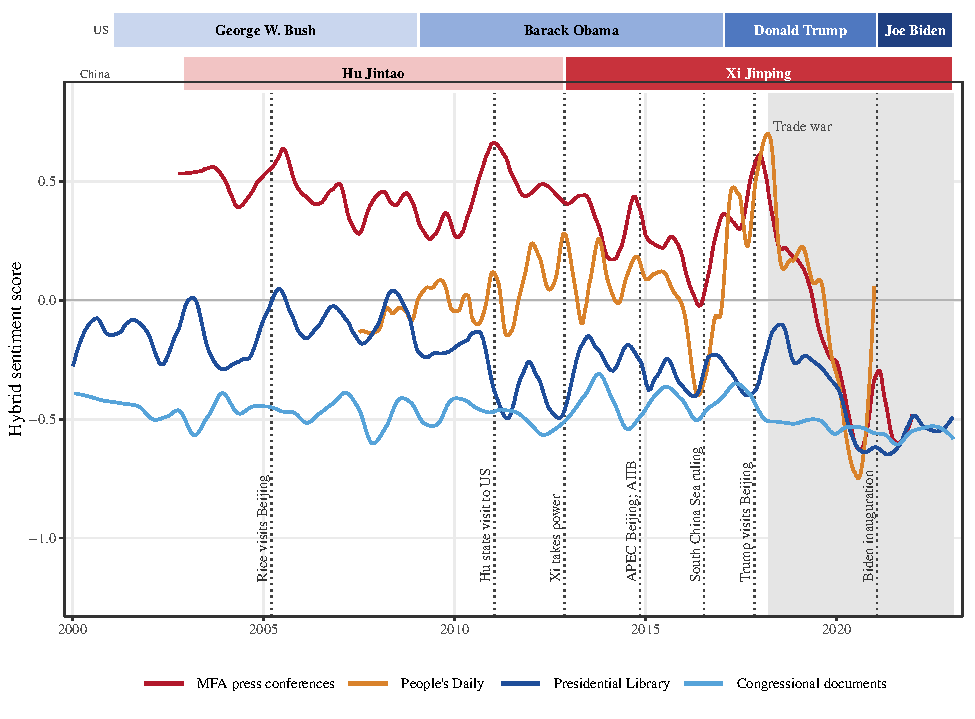
\includegraphics[width=\textwidth]{29_event_map.pdf}
  \caption{Sentiments of each country annotated with salient events}
  \label{fig:event-map}
\end{figure}

Second, before Chinese sentiments plunged in 2018, Beijing's rhetoric vis-à-vis its counterpart was nearly always more positive than Washington's rhetoric towards Beijing.\footnote{Da Wei also identifies 2018 as the ``watershed year'' in the US-China competition \autocite[21]{da2019}.} Moreover, members of Congress have disseminated a steady stream of pessimism with regard to China. Compared to the relative optimism of the MFA press corpus (at least until 2018), discussions of the US in \emph{People's Daily} also seem to be weighed down by noticeably more negativity. 

\subsection{Granger Causality with Time Filter}

When sentiments from the Chinese and US corpora are aggregated by week and cut forward from successive start dates, the Granger tests shift from bidirectional causality (start dates 2002--2007) to unidirectional causality with US data as the response (start dates 2008--2019). The F-test $p$-values from both directions of the test, as the start date is moved forward from 1 January 2002 to 1 January 2020, are laid out in the left panel of \cref{tab:granger-time}.\footnote{Here, we set a significance level of 0.05, and use a lag parameter of 3.}

% Generated by figures/13_14_24_25_granger_tables.R (score: a2) -- do not edit by hand.
% Requires \usepackage{booktabs} and \usepackage{threeparttable}.
\begin{table}[htbp]
\centering
\begin{threeparttable}
\caption{Granger causality between US and Chinese sentiment, by start date}
\label{tab:granger-time}
\small
\begin{tabular}{l rrr @{\hspace{1.5em}} rrr}
\toprule
 & \multicolumn{3}{c}{Full data} & \multicolumn{3}{c}{MFA / Presidential} \\
\cmidrule(lr){2-4}\cmidrule(lr){5-7}
Data after & US as & China as & Weeks & US as & China as & Weeks \\
 & response & response &  & response & response &  \\
\midrule
2002 (full series) & \textbf{$<$0.001} & \textbf{0.014} & 879 & \textbf{$<$0.001} & 0.128 & 648 \\
2003 & \textbf{$<$0.001} & \textbf{0.016} & 872 & \textbf{$<$0.001} & 0.125 & 644 \\
2004 & \textbf{$<$0.001} & \textbf{0.016} & 835 & \textbf{$<$0.001} & 0.102 & 612 \\
2005 & \textbf{$<$0.001} & \textbf{0.006} & 797 & \textbf{$<$0.001} & 0.051 & 580 \\
2006 & \textbf{$<$0.001} & \textbf{0.008} & 757 & \textbf{$<$0.001} & 0.075 & 545 \\
2007 & \textbf{$<$0.001} & \textbf{0.041} & 715 & \textbf{0.002} & 0.209 & 509 \\
2008 & \textbf{$<$0.001} & 0.129 & 669 & \textbf{0.003} & 0.434 & 480 \\
2009 & \textbf{$<$0.001} & 0.164 & 619 & \textbf{0.006} & 0.543 & 450 \\
2010 & \textbf{0.001} & 0.184 & 570 & \textbf{0.003} & 0.649 & 421 \\
2011 & \textbf{0.002} & 0.311 & 521 & \textbf{0.005} & 0.929 & 388 \\
2012 & \textbf{0.003} & 0.242 & 471 & \textbf{$<$0.001} & 0.884 & 365 \\
2013 & \textbf{$<$0.001} & 0.159 & 427 & \textbf{$<$0.001} & 0.862 & 347 \\
2014 & \textbf{0.002} & 0.231 & 382 & \textbf{$<$0.001} & 0.970 & 321 \\
2015 & \textbf{$<$0.001} & 0.189 & 341 & \textbf{$<$0.001} & 0.871 & 293 \\
2016 & \textbf{0.004} & 0.076 & 295 & \textbf{0.005} & 0.274 & 257 \\
2017 & \textbf{0.011} & 0.104 & 249 & \textbf{0.021} & 0.352 & 225 \\
2018 & \textbf{0.005} & 0.151 & 202 & \textbf{0.001} & 0.093 & 187 \\
2019 & \textbf{0.017} & 0.160 & 152 & \textbf{0.009} & \textbf{0.026} & 142 \\
2020 & 0.348 & 0.765 & 100 & 0.454 & 0.473 & 93 \\
\bottomrule
\end{tabular}
\begin{tablenotes}[flushleft]
\footnotesize
\item \textit{Notes:} Wald test $p$-values of bivariate Granger causality tests with 3 lags of each series. ``US as response'' tests whether lagged Chinese sentiment improves the prediction of US sentiment beyond lagged US sentiment; ``China as response'' tests the reverse. Bold: $p < 0.05$. Sentiment is the mean hybrid score (approach 2) of the documents in each period. Each pair of series is first tested for a unit root (augmented Dickey--Fuller, constant and trend, 5\% level, full sample). If both series are stationary, the test is run in levels; if neither is, on first differences; if only one is, by the Toda--Yamamoto procedure (both series in levels with one additional, untested lag of each). All $p$-values are from $F$-tests. Each row uses the weeks after 1 January of the year shown; the MFA series begins in October 2002, so the first row covers the full overlap. Weeks are seven-day bins counted from 1 January 2000; a week enters when both series have at least one document. Full data: US, Presidential Library documents and a random sample of 2,000 Congressional documents; China, MFA press conference answers and People's Daily articles. MFA / Presidential: US, dated Presidential Library documents; China, dated MFA press conference answers. Every weekly series is stationary, so all tests are in levels.
\end{tablenotes}
\end{threeparttable}
\end{table}


Additionally, because the MFA and the White House enjoy the greatest proximity to the foreign policy-making apparatus in Beijing and Washington, their sentiments may both be more directly comparable and more representative of how core decision-makers perceived each other. Thus, I run another set of Granger tests on time series isolating these two corpora.

The F-test $p$-values of Granger causality tests using MFA and Presidential Library subsets are laid out in the right panel of \cref{tab:granger-time}.

What becomes evident in \cref{tab:granger-time} is that for the majority of time periods, the Granger causality tests exhibit unidirectional causality whereby Chinese sentiments effectively forecast US sentiments, but \emph{not} vice versa. In the MFA and Presidential Library series, this holds for every start date from 2002 through 2018: White House discourse about China seems to exhibit sentiments that ``react'' to the tones of MFA rhetoric towards the US. This result largely persists when we group sentiments into monthly instead of weekly time series (\cref{fig:granger-tree-findings}).

Granger causality tests constructed from backward-dating temporal cuts, by contrast, were rarely significant. This finding indicates that the predictive power of US and Chinese political sentiments towards each other is much more salient in more recent periods of time.

\subsection{Granger Causality with Topic Filters}

\subsubsection*{Exploring Time Series by Topic}

Beyond applying Granger causality on sentiment trends filtered longitudinally, it is also possible to look at how sentiment trends for specific topics or themes correlate with one another.

First, by applying the filters introduced in the topic-keyword dyad table above (\cref{tab:topic-keywords}), we can visualize how the relative popularity of each issue area fluctuates over time. \Cref{fig:topic-counts} illustrates how often references to trade, the Chinese domestic periphery, multilateral negotiations, Taiwan, global health, the South China Sea, and Russia surface in US documents (top panel) and in Chinese discourse vis-à-vis the US (bottom panel) over time. Each topic is denoted by a band in a stacked area plot, and the formerly irregular and jagged contours of the area chart have been, once again, smoothed by LOESS.\footnote{Many documents mention two or more topics. These are counted once per topic in the area chart, although this does not affect the subsequent analysis. Topics within the figure are ordered as in \cref{tab:topic-keywords}, not by their relative salience.}

\begin{figure}[!htbp]
  \centering
  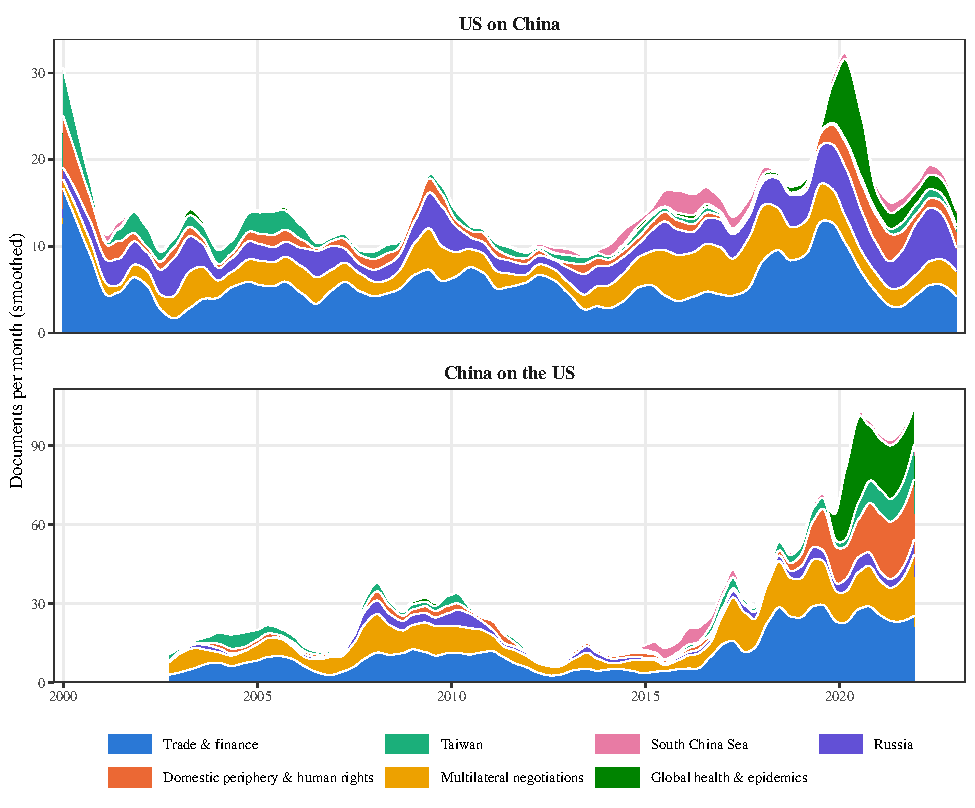
\includegraphics[width=\textwidth]{15_16_topic_counts.pdf}
  \caption{Document counts by topic over time, US and China data}
  \label{fig:topic-counts}
\end{figure}

Several key takeaways can be immediately gleaned from these plots. First, trade and finance has been the most frequent topic in government discourse surrounding US-China relations for most of the past two decades. In the US, we see ``bursts'' of mentions related to this motif around 2000, as well as between roughly 2018 and 2020. Both spikes make intuitive sense: the former coincides with the debate over China's accession to the World Trade Organization (and Congress's 2000 vote to grant China permanent normal trade relations), whereas the latter signals the onset of the trade war that broke out in early 2018.\footnote{For informative overviews and chronologies of the US-China relationship, particularly with regard to trade, see \textcite{brown2018} and \textcite{wang2019}.} While the Chinese data do not extend back far enough to capture discourse surrounding WTO entry, we do observe a similar jump beginning in 2017 and intensifying from 2018.

Another feature to point out in the bottom panel of \cref{fig:topic-counts} is that domestic periphery controversies---perhaps the most sensitive issue for Chinese policy-makers---moved into the rhetorical spotlight starting in late 2018. This burst in mentions could be driven by a number of factors, ranging from the pro-democracy movement in Hong Kong to the atrocities in Xinjiang. The surge of domestic periphery issues to the forefront of Chinese discourse (i.e.\ an increase in their share of documents) coincides with a pronounced decline in Chinese sentiments vis-à-vis the US (\cref{fig:china-periphery}).\footnote{For a clear explanation of China's sensitivity around issues related to territorial integrity, see \textcite[193--200]{nathan2015}.}

\begin{figure}[!htbp]
  \centering
  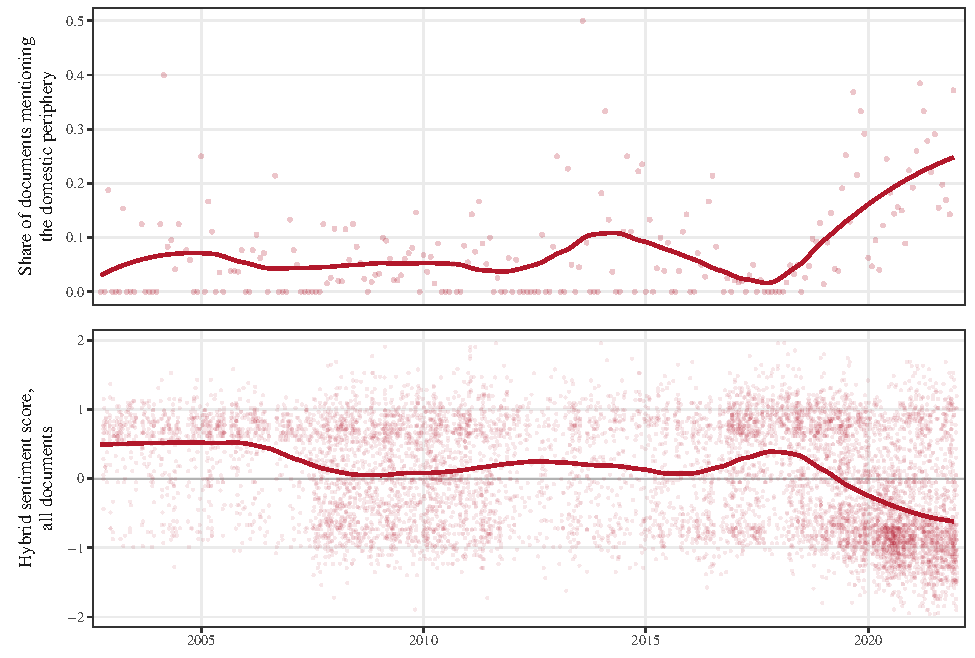
\includegraphics[width=\textwidth]{17_china_periphery_sentiment.pdf}
  \caption[Domestic periphery mentions and sentiment, China data]{Domestic periphery mentions and sentiment, China data. Top: monthly share of Chinese documents mentioning the domestic periphery; bottom: hybrid sentiment scores of all Chinese documents. Curves are LOESS fits.}
  \label{fig:china-periphery}
\end{figure}

\Cref{fig:topic-sent} disaggregates the tone of US and Chinese discourse by topic, plotting both countries' sentiment series together in each topic's panel. In most topics, Chinese sentiment sits above US sentiment for much of the period before converging towards it in the late 2010s.

\begin{figure}[!htbp]
  \centering
  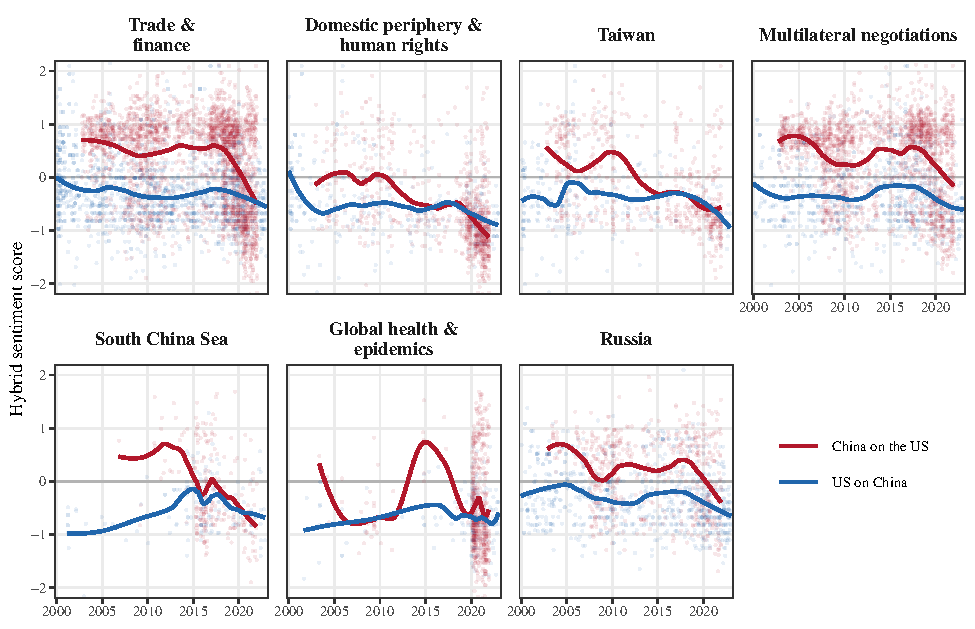
\includegraphics[width=\textwidth]{18_19_topic_sentiment.pdf}
  \caption{US and Chinese document sentiments by topic}
  \label{fig:topic-sent}
\end{figure}

\subsubsection*{Granger Causality}

Having visualized sentiment trends disaggregated by issue area, I run Granger tests on each topic's pair of time series. The F-test results are reported in \cref{tab:granger-topics}. Over the full time series, topic-specific Granger causality tests only return significant results for ``trade and finance'' (US as response) and ``global health'' (China as response). In the period since 2015, when MFA data becomes denser, the US-as-response test for ``trade and finance'' remains significant, as shown in the right panel of \cref{tab:granger-topics}. Unlike in the all-topic specifications, however, per-topic Granger causality tests do not show robust unidirectional statistical significance with the US as response, which partly reflects the sparsity of the data after applying topic filters.

% Generated by figures/13_14_24_25_granger_tables.R (score: a2) -- do not edit by hand.
% Requires \usepackage{booktabs} and \usepackage{threeparttable}.
\begin{table}[htbp]
\centering
\begin{threeparttable}
\caption{Granger causality between US and Chinese sentiment, by topic}
\label{tab:granger-topics}
\small
\begin{tabular}{l rrr @{\hspace{1.5em}} rrr}
\toprule
 & \multicolumn{3}{c}{All years} & \multicolumn{3}{c}{After 2015} \\
\cmidrule(lr){2-4}\cmidrule(lr){5-7}
Topic & US as & China as & Months & US as & China as & Months \\
 & response & response &  & response & response &  \\
\midrule
Domestic periphery \& human rights$^{b}$ & 0.268 & 0.066 & 87 & 0.630 & 0.785 & 42 \\
Multilateral negotiations & 0.443 & 0.243 & 201 & \textbf{0.043} & 0.139 & 80 \\
Trade \& finance & \textbf{0.043} & 0.555 & 217 & \textbf{0.013} & 0.898 & 79 \\
Taiwan$^{b}$ & 0.426 & 0.636 & 69 & 0.963 & \textbf{0.041} & 22 \\
South China Sea$^{a}$ & 0.376 & 0.938 & 45 & 0.441 & 0.975 & 36 \\
Global health \& epidemics$^{a}$ & 0.807 & \textbf{0.042} & 27 & 0.145 & 0.504 & 22 \\
Russia & 0.379 & 0.352 & 147 & \textbf{0.045} & \textbf{0.027} & 69 \\
\bottomrule
\end{tabular}
\begin{tablenotes}[flushleft]
\footnotesize
\item \textit{Notes:} Wald test $p$-values of bivariate Granger causality tests with 3 lags of each series. ``US as response'' tests whether lagged Chinese sentiment improves the prediction of US sentiment beyond lagged US sentiment; ``China as response'' tests the reverse. Bold: $p < 0.05$. Sentiment is the mean hybrid score (approach 2) of the documents in each period. Each pair of series is first tested for a unit root (augmented Dickey--Fuller, constant and trend, 5\% level, full sample). If both series are stationary, the test is run in levels; if neither is, on first differences; if only one is, by the Toda--Yamamoto procedure (both series in levels with one additional, untested lag of each). All $p$-values are from $F$-tests. Each series is the monthly mean score of the documents matching a topic's keywords (full US and Chinese data). Months in which either country has no document on the topic are dropped before lagging; ``Months'' counts the months left. The right panel uses only months after 1 January 2015. The test for each topic is chosen on all months and kept for the right panel. $^{a}$ First differences. $^{b}$ Toda--Yamamoto. Other rows: levels.
\end{tablenotes}
\end{threeparttable}
\end{table}


\subsection{Overview of Meaningful Findings}

In most Granger causality tests examined in my research, Chinese sentiment trends appear to meaningfully forecast US time series, whereas US data is much less effective in forecasting Chinese sentiments. \Cref{fig:granger-tree-findings} summarizes all Granger causality specifications and their directional significance. These patterns suggest that sentiment time series constructed from US foreign policy discourse frequently track lagged features of the Chinese data. The natural reading is that Chinese political discourse tends to set sentiment trends while US discourse tends to react to them---a reading that \cref{sec:limitations} qualifies.

\begin{figure}[!htbp]
  \centering
  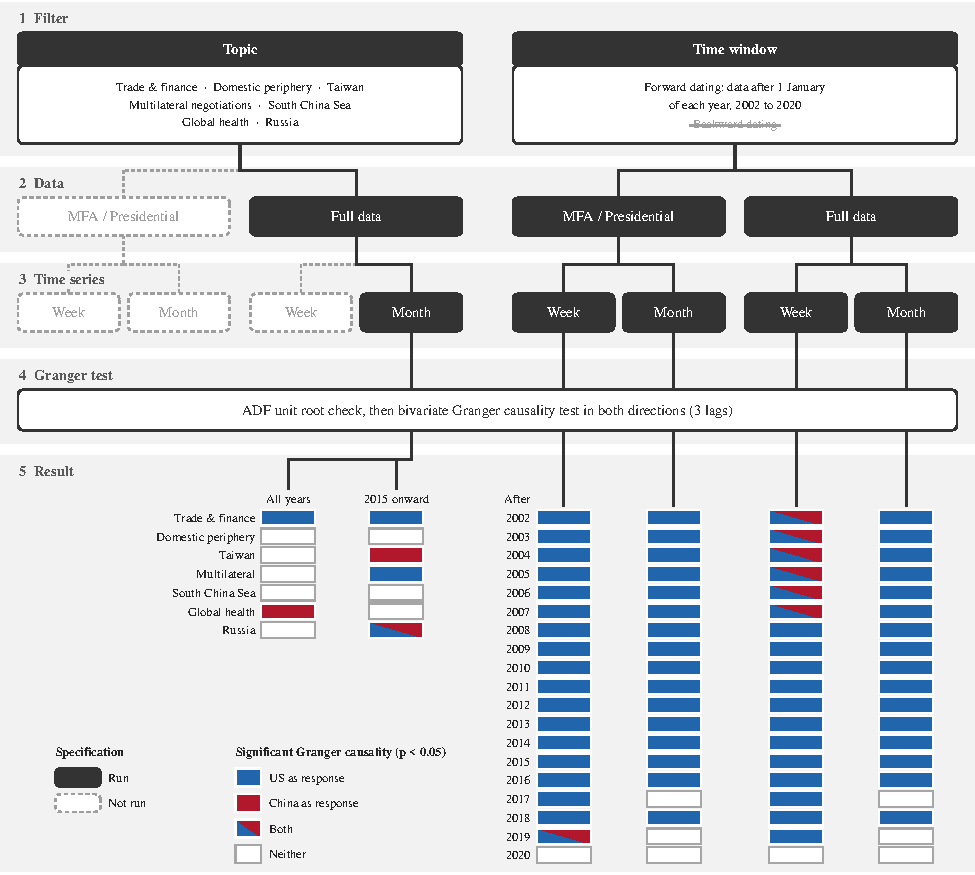
\includegraphics[width=\textwidth]{28_granger_tree_findings.pdf}
  \caption[Bivariate Granger causality tree with summary of findings]{Bivariate Granger causality tree with summary of findings. Each cell reports which direction of the Granger test is significant at $p < 0.05$ (3 lags). Topic series use the full data aggregated by month, over all years and from 2015 onward (\cref{tab:granger-topics}); time-window series use forward-dating cuts at the start of each year.}
  \label{fig:granger-tree-findings}
\end{figure}

% =====================================================================

\section{Limitations}
\label{sec:limitations}

\subsection{Time Series Noise Compromises Granger Causality Tests}

When interpreting the significance of the US-as-response Granger causality tests, it is important to note that the US time series is much noisier than its Chinese counterpart. 

We can illustrate this by computing a ``signal-to-noise ratio'' within the China and US time series. Consider the set-up in \cref{eq:avg}, where $\bar y_{c,t} = \theta_{c,t} + \bar\varepsilon_{c,t}$ (dropping the speaker or source effects term). Given that $\theta_{c,t}$ is held fixed within each time period, the variance in sentiments across documents in $t$ is entirely driven by noise. We can therefore take a pooled average of the within-period variance of document sentiments to estimate the document-level noise variance, $\sigma_c^2$. The mean sentiment in period $t$ then has noise variance $\sigma_c^2/n_{c,t}$, where $n_{c,t}$ is the number of documents in $t$. Averaged over periods, the noise variance of $\bar y_{c,t}$ is therefore
\begin{align}
  \tau_c^2 \equiv \sigma_c^2 \cdot \mathbb E\!\left[1/n_{c,t}\right].
\end{align}
Assuming that signal and noise are uncorrelated, we have $\mathrm{Var}(\bar y_{c,t}) = \mathrm{Var}(\theta_{c,t}) + \tau_c^2$. The signal-to-noise ratio, $\mathrm{Var}(\theta_{c,t}) / \tau_c^2$, of both countries' weekly time series is reported in \cref{tab:noise-snr}.

% Generated by robustness/noise_granger.R (Part 4) -- do not edit by hand.
% Requires \usepackage{booktabs} and \usepackage{threeparttable}.
\begin{table}[htbp]
\centering
\begin{threeparttable}
\caption{Signal-to-noise ratio of the weekly sentiment series}
\label{tab:noise-snr}
\small
\begin{tabular}{l rrr}
\toprule
 & Signal-to-noise & Documents & Weeks with \\
 & ratio & per week (mean) & one document \\
\midrule
\multicolumn{4}{l}{\textit{Panel A: Full country series} (879 weeks)} \\
\quad United States & 0.34 & 4.4 & 109 (12\%) \\
\quad China & 1.04 & 9.3 & 50 (6\%) \\
\addlinespace
\multicolumn{4}{l}{\textit{Panel B: MFA vs.\ Presidential Library} (648 weeks)} \\
\quad Presidential Library & 0.30 & 3.2 & 204 (31\%) \\
\quad MFA press conferences & 0.88 & 8.0 & 64 (10\%) \\
\bottomrule
\end{tabular}
\begin{tablenotes}[flushleft]
\footnotesize
\item \textit{Notes:} Signal-to-noise ratio is $\widehat{\mathrm{Var}}(\theta_{c,t})/\hat\tau_c^2$, where $\hat\sigma_c^2$ is the pooled within-week variance of document scores, $\hat\tau_c^2 = \hat\sigma_c^2 \cdot \overline{1/n_{c,t}}$, and $\widehat{\mathrm{Var}}(\theta_{c,t}) = \widehat{\mathrm{Var}}(\bar y_{c,t}) - \hat\tau_c^2$. Weeks are those in which both series of a panel have at least one document, the samples of the Granger tests in the left (Panel A) and right (Panel B) panels of \cref{tab:granger-time}. Weeks with one document add nothing to $\hat\sigma_c^2$ and are the noisiest weeks of the series. Panel A: US = Presidential Library and a random sample of 2,000 Congressional documents; China = MFA press conference answers and \emph{People's Daily} articles. Sentiment is the hybrid score (approach 2).
\end{tablenotes}
\end{threeparttable}
\end{table}


This ratio is roughly a third as large for the US time series as for the Chinese one, in large part because the US dataset is sparser, and the signal-to-noise ratio is increasing in the number of documents per week, $n_{c,t}$. 

Assuming that latent signals persist over time, a noisier measure of the past signal is a weaker predictor of future signals. Thus, if the US and China time series are driven by the same underlying ``temperature'' (plausible given they are responding to the same set of world events), then $\bar{y}_{\mathrm{US},t-n}$ will only noisily forecast $\bar{y}_{\mathrm{US},t}$. On the other hand, the cleaner $\bar{y}_{\mathrm{CN},t-n}$ will be a better predictor of $\bar{y}_{\mathrm{US},t}$. A US-as-response Granger causality test will therefore find a relatively large reduction in RSS from the restricted to the full model. In other words, when one time series is substantially noisier than the other, it is possible that a Granger causality test will find spurious significance when the noisier time series is the response variable. Future work can consider whether the Granger causality test asymmetry persists when we downsample the Chinese time series each week, or use state-space models to better capture latent signals.

\subsection{Stance vs.\ Sentiment}
\label{sec:stance}

The current hybrid sentiment classifier considers the sentiment of a document as a whole, whereas a better approach would consider the sentiment of a document produced by country $c$ with respect to country $c'$. 

As a case in point, consider MFA spokesperson Wang Wenbin's exchange with a reporter on February 22, 2021 with regard to the JCPOA: 

\begin{displayquote}
  China welcomes and commends [IAEA verification activities] and hopes that the two sides continue to work toward the same direction and earnestly follow through on this consensus. We also call on relevant sides to play a constructive role in this process. China holds that the return of the United States to the JCPOA is the only correct approach to resolve the impasse on the Iranian nuclear issue.
\end{displayquote}

While the document overall lauds multilateral cooperation towards a nuclear deal, and thus gets a positive sentiment score, Wang is directing veiled criticism towards the US for its withdrawal from the JCPOA. Thus, the document's stance towards the US is negative. A more nuanced stance classifier can take a two-step approach: first, it identifies whether a document from country $c$ is directed at country $c'$; then, it classifies the sentiment of the document with respect to country $c'$.

% =====================================================================
\section{Discussion of Key Findings}
\label{sec:discussion}

\subsection{What Are Ways to Explain Foreign Policy Discourse?}

\subsubsection*{A. Discourse as a Reflection of Reality}

The most straightforward interpretation of foreign policy discourse for the purposes of this paper, of course, is simply that rhetoric is a good proxy for how policymakers from one country perceive their counterparts, and for the actual warmth of bilateral ties. This explanation is informed by Biwu Zhang's \emph{Chinese Perceptions of the US} \autocite*{zhang2011}, as well as David Shambaugh's \emph{Beautiful Imperialist} \autocite*{shambaugh1991}, which both enlist elite discourse ranging from state-affiliated academic publications to newspapers as a medium that reflects the abstract concept of how China perceives the US.

Under this explanation, the patterns of interaction picked up by Granger models serve as a proxy for the relationship between how the US perceives the state of its relationship with China, and vice versa. In this sense, the US's more ``reactive'' posture vis-à-vis Chinese sentiment trends suggests that China is often the first to perceive upturns, tensions, and discord in bilateral ties. However, we must be careful not to over-extend this insight about perceptions and rhetoric to claim that China is provocative in its diplomatic practice.

\subsubsection*{B. Discourse as a Constitutive and Productive Player}

While explanation \emph{A} encompasses a traditional understanding of foreign policy discourse as a passive reflection of reality, explanation \emph{B} lends an ear to critical discourse analysis (CDA) and identifies discourse as a site where norms and meanings are actively constituted. Jennifer Milliken identifies two characteristics of discourse as viewed from a constructivist perspective---that it acts ``as a system of signification'' which can ``construct social realities,'' and that it is imbued with ``productivity,'' which at times means ``operationalizing a particular regime of truth'' \autocite[229]{milliken1999}.

% COMMENT (Berlinerblau), on "it is an active participant": This section seems like
% a bit of a different paper. Different questions. Not sure what advice I have
As such, foreign policy discourse is not just a transparent looking glass through which geopolitical truths are reflected; rather, it is an active participant in international relations in its own right that can signal and produce new norms, new behaviors, and new roles.

A case in point here is the reconstitution of Chinese foreign policy discourse under the Hu Jintao administration. For the preceding two decades, China had been operating under a ``minimalist'' foreign policy doctrine encapsulated by Deng's slogans ``hiding and biding'' (韬光养晦), as well as ``not taking the lead'' (不当头). However, China's rapid growth, coupled with an increasingly complex external environment, pushed Beijing to search for a new \emph{modus operandi} in the international arena. In this sense, Hu's new umbrella slogan for Chinese diplomacy, ``harmonious world'' (和谐世界), signaled to the world that China was ready to come out of its metaphorical shell and enter a new developmental stage. Hu's foreign policy discourse, therefore, is not just a straightforward reflection of Chinese ambitions, but it is actively constituting a new role for the country to grow into. ``Harmonious world,'' and by extension Xi's ``community of common destiny'' (命运共同体), signal new geopolitical norms that China is trying to construct \autocite[29--32]{su2009}.

Similarly, on the American side, the Obama-era mantra ``pivot to Asia,'' as well as the idea of ``America's Pacific Century'' (which crystallized in a \emph{Foreign Policy} essay penned by Secretary Clinton), both actively sought to construct new realities on the ground \autocite{clinton2011}. The ``pivot,'' therefore, constitutes a signpost orienting America towards a more proactive and enhanced presence in the Asia-Pacific theater \autocite{davidson2014}. Similar to Hu's ``harmonious world'' or Xi's ``common destiny,'' the Obama administration's foreign policy discourse has actively produced new norms and new dynamics within US-China diplomacy.

From this viewpoint, discourse is imbued with a sort of power to constitute and legitimize ``new regimes of truth.'' According to Semenov and Tsvyk, moreover, Chinese policymakers pay particularly close attention to their ``discourse power'' (话语权), which represents their ability to speak up on the international stage to popularize and legitimize their narratives and their worldviews \autocite[566]{semenov2021}.

Given the norm-constituting powers of words, China's role as a ``trend-setter'' in foreign policy sentiments may put it in a position to shape the terms of bilateral discourse and harness its constitutive power.

\subsubsection*{C. Discourse as Performance and Theater}

Explanations \emph{A} and \emph{B} both imply that the Granger tests capture something meaningful about bilateral relations. This third explanation, on the other hand, acknowledges exogenous factors that may complicate the interpretation of my results. Namely, foreign policy discourse can, at times, be detached from foreign policy practices because it not only serves reflective, communicative, or norm-setting functions, but it is also highly \emph{performative}.

For instance, discourse can serve this theatrical performance function for a country's broad populace. According to Sullivan and Wang, Hua Chunying's brand of fiery foreign policy discourse (prominent in MFA press conferences during the Trump years) is incentivized by ``cyber-nationalist'' pressures emanating from the bottom up \autocite{sullivan2023}. But discourse does not always correspond to actual practice. Poh and Li argue that the Xi administration's increasingly ambitious slogans, threats, and promises mask substantial continuity in foreign policy between Xi and his more restrained predecessors \autocite[95--97]{poh2017}.

What's more, a policymaker's rhetoric can also serve performative purposes for colleagues or superiors. Notably, an increasingly popular theory among China watchers is that faced with a slew of bureaucratic pressures, the MFA needed to deploy its most firebrand ``wolf warriors'' to the front lines of political discourse in order to avoid being shunted into irrelevance.

% PORT: "National Development and Reform Corporation" -> "Commission".
According to Zhao and Gao, as well as Jing Sun, the embattled MFA is being squeezed by bureaucratic pressures from all sides. For one, Xi is centralizing the decision-making pipeline by setting up Leading Small Groups (LSGs) with himself at the nexus, while sidelining the MFA. At the same time, other agencies like the Ministry of Commerce (MOFCOM), the National Development and Reform Commission (NDRC), and the People's Liberation Army have been encroaching upon the MFA's turf \autocites[420, 422]{sun2017}[47]{zhao2015}. To stay afloat, the agency has resorted to jingoistic outbursts on the international stage to showcase its loyalty, as well as its ability to follow Xi's vision to the letter. As Peter Martin puts it in \emph{China's Civilian Army}, the virulent ``Wolf Warrior'' rhetoric stems from the diplomatic corps being ``unable to extricate themselves from the constraints of a secretive, paranoid political system which rewards unquestioning loyalty and ideological conviction'' \autocite[5]{martin2021}.

This bureaucratic turf wars theory also lends some credence to the idea that foreign policy discourse may not fully adhere to explanations \emph{A} and \emph{B}, and that it is important to factor exogenous and domestic variables into the research calculus.

% =====================================================================
\section{Applications and Future Work}
\label{sec:future}

\subsection{A Cheap Yet Effective Relationship Monitor?}

Interpreting political discourse through NLP and time-series analysis is useful because it provides a relatively cheap and interpretable proxy for the temperature of bilateral relations (as discussed in explanation \emph{A} in the previous section). By quantifying the emotional valence of the two countries' foreign policy discourse, it is possible to create a bilateral relations ``thermometer'' that takes readings at fine time intervals while also revealing long-run trends.

To be sure, more and more scholars and institutions are trying to publish their own relationship monitors. Morning Consult, for example, curates and regularly updates a US-China Relations Barometer, which derives the positivity of US perceptions towards China (or vice versa) based on iterative polling of the general populace \autocite{morningconsult}. 

However, gauging the temperature of the multifaceted ties between the US and China through surveys is time-consuming and potentially expensive work. The survey methodology runs into further obstacles when we try to move from studying relatively more accessible public opinion to piercing the veil of secrecy that often shrouds policymakers' opinion. These problems are compounded when we try to expand our inquiry about the evolution of bilateral relations over two or more decades.

This paper builds on the existing literature on foreign policy discourse and perceptions by developing a fast, efficient, long-term, and high-resolution relationship monitor. By gathering a large set of texts pertinent to the US-China relationship and feeding them into a sentiment analysis pipeline, I generate quantifiable and granular measures of the warmth of bilateral ties spanning extensive time frames.

\subsection{The Long and Promising Road Ahead}

Of course, the relationship monitor introduced here needs considerable refinement before it becomes a mature tool. I see two paths for future research branching from this initial ``proof of concept.'' The first entails creating a larger and more comprehensive dataset. This means using greater computing resources to mine textual data pertaining to a wider range of foreign policy stakeholders, such as the Politburo, the State Council, and MOFCOM in China, the National Security Council along with State and Defense in the US, or even think tanks and authoritative voices in the academy in both states.

The second path along the future research roadmap entails conducting textual analysis with increasingly sophisticated methods. Sentiment classification, for example, can move beyond a single spectrum ranging from negative to positive valence. We could also code emotional frames such as anger, surprise, or hope, or more complex themes such as persuasion, threat perception, or ambivalence. Beyond situating texts along a tonal spectrum, it is also useful to consider how \emph{stances} (i.e.\ affirmation or negation regarding a particular political issue or entity) are reflected within different texts, as discussed in \cref{sec:stance}.

These enhanced classifiers could draw on transformer-based language models, from fine-tuned BERT classifiers to large language models.

\subsection{Piercing the Veil of Perception}

In \emph{Perception and Misperception}, Robert Jervis points out that a security dilemma, at its essence, can be traced back to the challenge of understanding mutual perceptions between two states \autocite[xv]{jervis2017}. In this sense, the ``original sin'' spoiling US-China rapport is a psychology of distrust and suspicion that thrives amidst an environment of uncertainty.

Andrew Scobell, applying Jervis to US-China relations, remarks that both states are domestically preoccupied, struggle with ``chronic empathy deficiency,'' and thus are growing alarmed by elevated threat perceptions as their power differentials shrink \autocite[664]{scobell2020}.

A data-driven relationship monitor could reduce perceptual uncertainties by drawing on large volumes of text containing what the US and Chinese governments say about each other. By parsing and synthesizing many accessible data points that only imperfectly represent bilateral perceptions, it is possible to \emph{estimate} the latent perceptions underlying the US-China stand-off.

% =====================================================================
\begin{singlespace}
\setlength{\bibitemsep}{0.6\baselineskip}
\printbibliography[title={References}]
\end{singlespace}

\end{document}
